Kista enables the export of a TiKZ file which reflects the KisTA model.
%
The export can be done regardless the model has been captured through the
the C/C++ API or the KisTA XML front-end.

\subsubsection{Using C++ API}
\label{sec:sketch_report_cpp_api}

Listing~\ref{list:sketch_report_class} shows the API that the user can use for enabling and controlling the export of a system sketch.

%\begin{table}[t]
\begin{lstlisting}[style=KistaCodeStyle,caption={API for controling tracing tasks and scheduler activity.},label=list:sketch_report_class]

class sketch_report_t : sc_module {
	friend sketch_report_t& operator<<(sketch_report_t& sk_rpt, std::string content);
public:
		// create sketch report class, by default disabled
		// sketch file with the default name "system_sketch"
	sketch_report_t();
	
	bool &is_enabled(); // true if sketch reported enabled
	
		// set name of sketch report file
	void set_file_name(std::string	name_par); 
	
	void enable(); // enable sketch report and creates report header
	                // (has to be called at construction time and after set_name, otherwise, settled name is overriden and the default one taken)
	
	// configuration of the draw
	void draw_sys_level_conn();
	
	void highlight_environment();
	void highlight_system();      // overrides the hilighting of application and platform
	void highlight_application();
	void highlight_platform();

        void only_image();
        void set_scale(float scale_par);

   ...
};

\end{lstlisting}
%\end{table}

When the user includes the "kista.h" header, a global element \texttt{sketch\_report} of type \texttt{sketch\_report\_t}
is immediately instanced.

In the simplest case, the user only needs to call the \texttt{enable()} method, before the \texttt{sc\_start()} method.
Then, to generate the sketch, it is necessary to lauch the KisTA executable.
The sketch is generated at the end of the elaboration.
Notice that it is not necessary to run the simulation.
By default, the file is generated with the name \texttt{system\_sketch.tex}.

The user can control the name of the sketch by means of the \texttt{set\_file\_name} method,
which has to be called before the call to the \texttt{enable()} method.

The method \texttt{is\_enabled()} serves to test if the sketch has been enabled.

Figure~\ref{fig:ex3_sketch} ilustrates the result of the sketch reported
after applying the \texttt{pdflatex} command to the \texttt{ex3\_sketch.tex} file
produced in the basic real-time example 3.
This example consists of two independent tasks mapped to a single local scheduler.
Notice that the reported sketch represents the default processing element
instanced by KisTA when the user does not explicitly specifies a processing element.
%

\begin{figure}[h]
\centering
%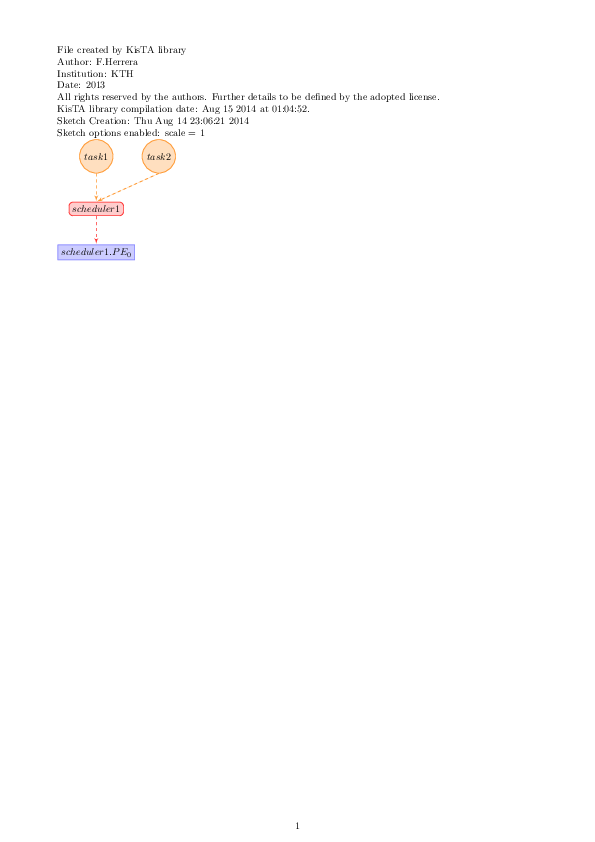
\includegraphics[width=\textwidth]{./figs/ex3_sketch.png} 
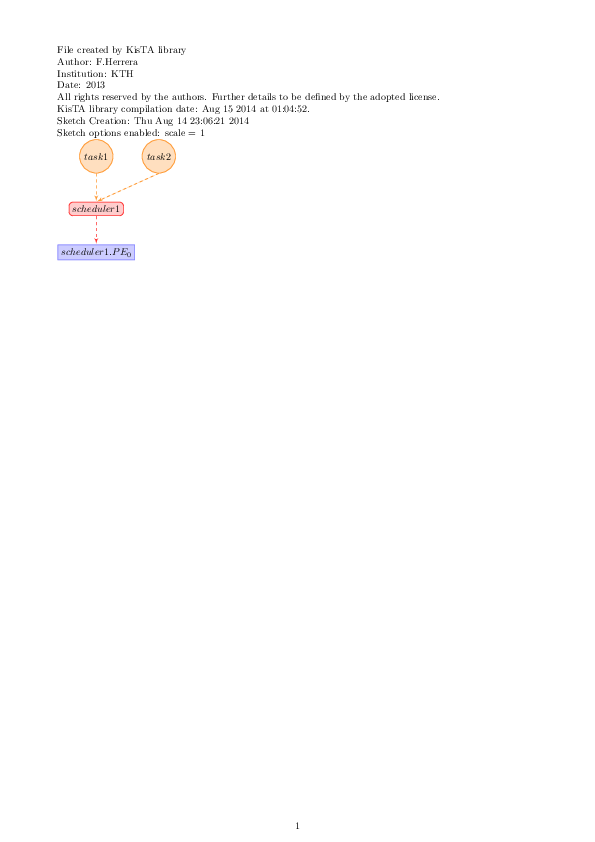
\includegraphics[width=0.75\textwidth]{./figs/ex3_sketch.png} 
\caption{Sketch report of basic RT example 3.} 
\label{fig:ex3_sketch}
\end{figure}

Notice that the export is also done for an A4 paper, and that a text report
with information about KisTA, and about the date of the report and reporting options
used is given by default.
The \texttt{only\_image()} method can be used for avoiding such textual report
associated to the image.
%
This can be used together with the method \texttt{set\_scale(float)} in order to 
generate a pdf image taking most of the paper size, and to reduce the need
for further transformations when converting to other formats.

Figure~\ref{fig:ex3_sketch_only_img} ilustrates the result of the \texttt{pdflatex} command
application after conveniently using \texttt{only\_image()} and \texttt{set\_scale(4.0)} 
in the same basic RT example 3.

\begin{figure}[h]
\centering
%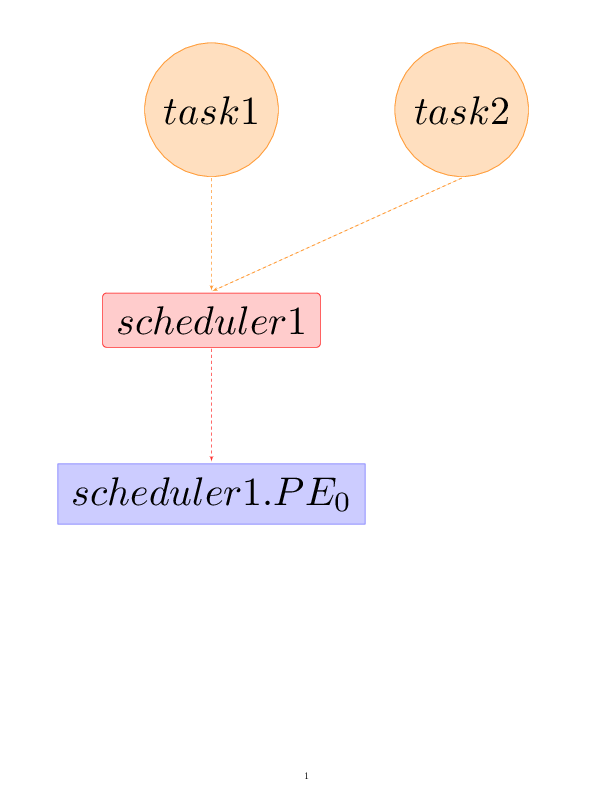
\includegraphics[width=\textwidth]{./figs/ex3_sketch_only_image_scale4.png} 
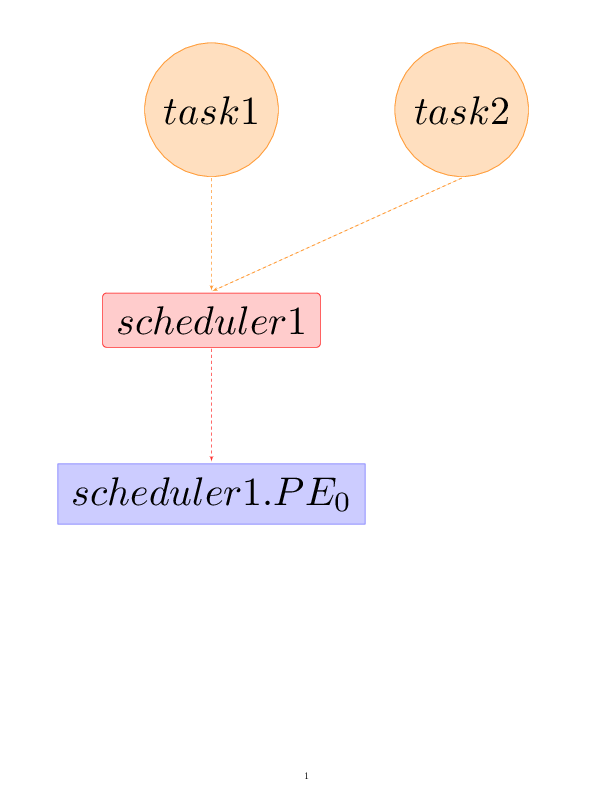
\includegraphics[width=0.75\textwidth]{./figs/ex3_sketch_only_image_scale4.png} 
\caption{Sketch report of basic RT example 3, configured to report only the image and with x4 scale} 
\label{fig:ex3_sketch_only_img}
\end{figure}


\subsubsection{Using the XML front-end}
\label{sec:sketch_report_xml}
